\documentclass{article}
\usepackage[utf8]{inputenc}
\usepackage[margin=1in]{geometry}
\usepackage{booktabs}
\usepackage{colortbl}
\usepackage{graphicx}
\usepackage{xcolor}
\usepackage{tikz}
\usepackage{pgfplots}
\begin{document}
\begin{center}
\section*{$z$-table (FPP style)}
%\begin{tabular}{lllllllllll}
\toprule
 & +0.00 & +0.01 & +0.02 & +0.03 & +0.04 & +0.05 & +0.06 & +0.07 & +0.08 & +0.09 \\
\midrule
0.0 & \cellcolor{gray!20}0.5000 & \cellcolor{gray!20}0.5040 & \cellcolor{gray!20}0.5080 & \cellcolor{gray!20}0.5120 & \cellcolor{gray!20}0.5160 & \cellcolor{gray!20}0.5199 & \cellcolor{gray!20}0.5239 & \cellcolor{gray!20}0.5279 & \cellcolor{gray!20}0.5319 & \cellcolor{gray!20}0.5359 \\
0.1 & 0.5398 & 0.5438 & 0.5478 & 0.5517 & 0.5557 & 0.5596 & 0.5636 & 0.5675 & 0.5714 & 0.5753 \\
0.2 & \cellcolor{gray!20}0.5793 & \cellcolor{gray!20}0.5832 & \cellcolor{gray!20}0.5871 & \cellcolor{gray!20}0.5910 & \cellcolor{gray!20}0.5948 & \cellcolor{gray!20}0.5987 & \cellcolor{gray!20}0.6026 & \cellcolor{gray!20}0.6064 & \cellcolor{gray!20}0.6103 & \cellcolor{gray!20}0.6141 \\
0.3 & 0.6179 & 0.6217 & 0.6255 & 0.6293 & 0.6331 & 0.6368 & 0.6406 & 0.6443 & 0.6480 & 0.6517 \\
0.4 & \cellcolor{gray!20}0.6554 & \cellcolor{gray!20}0.6591 & \cellcolor{gray!20}0.6628 & \cellcolor{gray!20}0.6664 & \cellcolor{gray!20}0.6700 & \cellcolor{gray!20}0.6736 & \cellcolor{gray!20}0.6772 & \cellcolor{gray!20}0.6808 & \cellcolor{gray!20}0.6844 & \cellcolor{gray!20}0.6879 \\
0.5 & 0.6915 & 0.6950 & 0.6985 & 0.7019 & 0.7054 & 0.7088 & 0.7123 & 0.7157 & 0.7190 & 0.7224 \\
0.6 & \cellcolor{gray!20}0.7257 & \cellcolor{gray!20}0.7291 & \cellcolor{gray!20}0.7324 & \cellcolor{gray!20}0.7357 & \cellcolor{gray!20}0.7389 & \cellcolor{gray!20}0.7422 & \cellcolor{gray!20}0.7454 & \cellcolor{gray!20}0.7486 & \cellcolor{gray!20}0.7517 & \cellcolor{gray!20}0.7549 \\
0.7 & 0.7580 & 0.7611 & 0.7642 & 0.7673 & 0.7704 & 0.7734 & 0.7764 & 0.7794 & 0.7823 & 0.7852 \\
0.8 & \cellcolor{gray!20}0.7881 & \cellcolor{gray!20}0.7910 & \cellcolor{gray!20}0.7939 & \cellcolor{gray!20}0.7967 & \cellcolor{gray!20}0.7995 & \cellcolor{gray!20}0.8023 & \cellcolor{gray!20}0.8051 & \cellcolor{gray!20}0.8078 & \cellcolor{gray!20}0.8106 & \cellcolor{gray!20}0.8133 \\
0.9 & 0.8159 & 0.8186 & 0.8212 & 0.8238 & 0.8264 & 0.8289 & 0.8315 & 0.8340 & 0.8365 & 0.8389 \\
1.0 & \cellcolor{gray!20}0.8413 & \cellcolor{gray!20}0.8438 & \cellcolor{gray!20}0.8461 & \cellcolor{gray!20}0.8485 & \cellcolor{gray!20}0.8508 & \cellcolor{gray!20}0.8531 & \cellcolor{gray!20}0.8554 & \cellcolor{gray!20}0.8577 & \cellcolor{gray!20}0.8599 & \cellcolor{gray!20}0.8621 \\
1.1 & 0.8643 & 0.8665 & 0.8686 & 0.8708 & 0.8729 & 0.8749 & 0.8770 & 0.8790 & 0.8810 & 0.8830 \\
1.2 & \cellcolor{gray!20}0.8849 & \cellcolor{gray!20}0.8869 & \cellcolor{gray!20}0.8888 & \cellcolor{gray!20}0.8907 & \cellcolor{gray!20}0.8925 & \cellcolor{gray!20}0.8944 & \cellcolor{gray!20}0.8962 & \cellcolor{gray!20}0.8980 & \cellcolor{gray!20}0.8997 & \cellcolor{gray!20}0.9015 \\
1.3 & 0.9032 & 0.9049 & 0.9066 & 0.9082 & 0.9099 & 0.9115 & 0.9131 & 0.9147 & 0.9162 & 0.9177 \\
1.4 & \cellcolor{gray!20}0.9192 & \cellcolor{gray!20}0.9207 & \cellcolor{gray!20}0.9222 & \cellcolor{gray!20}0.9236 & \cellcolor{gray!20}0.9251 & \cellcolor{gray!20}0.9265 & \cellcolor{gray!20}0.9279 & \cellcolor{gray!20}0.9292 & \cellcolor{gray!20}0.9306 & \cellcolor{gray!20}0.9319 \\
1.5 & 0.9332 & 0.9345 & 0.9357 & 0.9370 & 0.9382 & 0.9394 & 0.9406 & 0.9418 & 0.9429 & 0.9441 \\
1.6 & \cellcolor{gray!20}0.9452 & \cellcolor{gray!20}0.9463 & \cellcolor{gray!20}0.9474 & \cellcolor{gray!20}0.9484 & \cellcolor{gray!20}0.9495 & \cellcolor{gray!20}0.9505 & \cellcolor{gray!20}0.9515 & \cellcolor{gray!20}0.9525 & \cellcolor{gray!20}0.9535 & \cellcolor{gray!20}0.9545 \\
1.7 & 0.9554 & 0.9564 & 0.9573 & 0.9582 & 0.9591 & 0.9599 & 0.9608 & 0.9616 & 0.9625 & 0.9633 \\
1.8 & \cellcolor{gray!20}0.9641 & \cellcolor{gray!20}0.9649 & \cellcolor{gray!20}0.9656 & \cellcolor{gray!20}0.9664 & \cellcolor{gray!20}0.9671 & \cellcolor{gray!20}0.9678 & \cellcolor{gray!20}0.9686 & \cellcolor{gray!20}0.9693 & \cellcolor{gray!20}0.9699 & \cellcolor{gray!20}0.9706 \\
1.9 & 0.9713 & 0.9719 & 0.9726 & 0.9732 & 0.9738 & 0.9744 & 0.9750 & 0.9756 & 0.9761 & 0.9767 \\
2.0 & \cellcolor{gray!20}0.9772 & \cellcolor{gray!20}0.9778 & \cellcolor{gray!20}0.9783 & \cellcolor{gray!20}0.9788 & \cellcolor{gray!20}0.9793 & \cellcolor{gray!20}0.9798 & \cellcolor{gray!20}0.9803 & \cellcolor{gray!20}0.9808 & \cellcolor{gray!20}0.9812 & \cellcolor{gray!20}0.9817 \\
2.1 & 0.9821 & 0.9826 & 0.9830 & 0.9834 & 0.9838 & 0.9842 & 0.9846 & 0.9850 & 0.9854 & 0.9857 \\
2.2 & \cellcolor{gray!20}0.9861 & \cellcolor{gray!20}0.9864 & \cellcolor{gray!20}0.9868 & \cellcolor{gray!20}0.9871 & \cellcolor{gray!20}0.9875 & \cellcolor{gray!20}0.9878 & \cellcolor{gray!20}0.9881 & \cellcolor{gray!20}0.9884 & \cellcolor{gray!20}0.9887 & \cellcolor{gray!20}0.9890 \\
2.3 & 0.9893 & 0.9896 & 0.9898 & 0.9901 & 0.9904 & 0.9906 & 0.9909 & 0.9911 & 0.9913 & 0.9916 \\
2.4 & \cellcolor{gray!20}0.9918 & \cellcolor{gray!20}0.9920 & \cellcolor{gray!20}0.9922 & \cellcolor{gray!20}0.9925 & \cellcolor{gray!20}0.9927 & \cellcolor{gray!20}0.9929 & \cellcolor{gray!20}0.9931 & \cellcolor{gray!20}0.9932 & \cellcolor{gray!20}0.9934 & \cellcolor{gray!20}0.9936 \\
2.5 & 0.9938 & 0.9940 & 0.9941 & 0.9943 & 0.9945 & 0.9946 & 0.9948 & 0.9949 & 0.9951 & 0.9952 \\
2.6 & \cellcolor{gray!20}0.9953 & \cellcolor{gray!20}0.9955 & \cellcolor{gray!20}0.9956 & \cellcolor{gray!20}0.9957 & \cellcolor{gray!20}0.9959 & \cellcolor{gray!20}0.9960 & \cellcolor{gray!20}0.9961 & \cellcolor{gray!20}0.9962 & \cellcolor{gray!20}0.9963 & \cellcolor{gray!20}0.9964 \\
2.7 & 0.9965 & 0.9966 & 0.9967 & 0.9968 & 0.9969 & 0.9970 & 0.9971 & 0.9972 & 0.9973 & 0.9974 \\
2.8 & \cellcolor{gray!20}0.9974 & \cellcolor{gray!20}0.9975 & \cellcolor{gray!20}0.9976 & \cellcolor{gray!20}0.9977 & \cellcolor{gray!20}0.9977 & \cellcolor{gray!20}0.9978 & \cellcolor{gray!20}0.9979 & \cellcolor{gray!20}0.9979 & \cellcolor{gray!20}0.9980 & \cellcolor{gray!20}0.9981 \\
2.9 & 0.9981 & 0.9982 & 0.9982 & 0.9983 & 0.9984 & 0.9984 & 0.9985 & 0.9985 & 0.9986 & 0.9986 \\
3.0 & \cellcolor{gray!20}0.9987 & \cellcolor{gray!20}0.9987 & \cellcolor{gray!20}0.9987 & \cellcolor{gray!20}0.9988 & \cellcolor{gray!20}0.9988 & \cellcolor{gray!20}0.9989 & \cellcolor{gray!20}0.9989 & \cellcolor{gray!20}0.9989 & \cellcolor{gray!20}0.9990 & \cellcolor{gray!20}0.9990 \\
\bottomrule
\end{tabular}

\begin{tabular}{lllllllllll}
\toprule
 & +0.00 & +0.01 & +0.02 & +0.03 & +0.04 & +0.05 & +0.06 & +0.07 & +0.08 & +0.09 \\
\midrule
0.0 & \cellcolor{gray!20}0.0000 & \cellcolor{gray!20}0.0080 & \cellcolor{gray!20}0.0160 & \cellcolor{gray!20}0.0239 & \cellcolor{gray!20}0.0319 & \cellcolor{gray!20}0.0399 & \cellcolor{gray!20}0.0478 & \cellcolor{gray!20}0.0558 & \cellcolor{gray!20}0.0638 & \cellcolor{gray!20}0.0717 \\
0.1 & 0.0797 & 0.0876 & 0.0955 & 0.1034 & 0.1113 & 0.1192 & 0.1271 & 0.1350 & 0.1428 & 0.1507 \\
0.2 & \cellcolor{gray!20}0.1585 & \cellcolor{gray!20}0.1663 & \cellcolor{gray!20}0.1741 & \cellcolor{gray!20}0.1819 & \cellcolor{gray!20}0.1897 & \cellcolor{gray!20}0.1974 & \cellcolor{gray!20}0.2051 & \cellcolor{gray!20}0.2128 & \cellcolor{gray!20}0.2205 & \cellcolor{gray!20}0.2282 \\
0.3 & 0.2358 & 0.2434 & 0.2510 & 0.2586 & 0.2661 & 0.2737 & 0.2812 & 0.2886 & 0.2961 & 0.3035 \\
0.4 & \cellcolor{gray!20}0.3108 & \cellcolor{gray!20}0.3182 & \cellcolor{gray!20}0.3255 & \cellcolor{gray!20}0.3328 & \cellcolor{gray!20}0.3401 & \cellcolor{gray!20}0.3473 & \cellcolor{gray!20}0.3545 & \cellcolor{gray!20}0.3616 & \cellcolor{gray!20}0.3688 & \cellcolor{gray!20}0.3759 \\
0.5 & 0.3829 & 0.3899 & 0.3969 & 0.4039 & 0.4108 & 0.4177 & 0.4245 & 0.4313 & 0.4381 & 0.4448 \\
0.6 & \cellcolor{gray!20}0.4515 & \cellcolor{gray!20}0.4581 & \cellcolor{gray!20}0.4647 & \cellcolor{gray!20}0.4713 & \cellcolor{gray!20}0.4778 & \cellcolor{gray!20}0.4843 & \cellcolor{gray!20}0.4907 & \cellcolor{gray!20}0.4971 & \cellcolor{gray!20}0.5035 & \cellcolor{gray!20}0.5098 \\
0.7 & 0.5161 & 0.5223 & 0.5285 & 0.5346 & 0.5407 & 0.5467 & 0.5527 & 0.5587 & 0.5646 & 0.5705 \\
0.8 & \cellcolor{gray!20}0.5763 & \cellcolor{gray!20}0.5821 & \cellcolor{gray!20}0.5878 & \cellcolor{gray!20}0.5935 & \cellcolor{gray!20}0.5991 & \cellcolor{gray!20}0.6047 & \cellcolor{gray!20}0.6102 & \cellcolor{gray!20}0.6157 & \cellcolor{gray!20}0.6211 & \cellcolor{gray!20}0.6265 \\
0.9 & 0.6319 & 0.6372 & 0.6424 & 0.6476 & 0.6528 & 0.6579 & 0.6629 & 0.6680 & 0.6729 & 0.6778 \\
1.0 & \cellcolor{gray!20}0.6827 & \cellcolor{gray!20}0.6875 & \cellcolor{gray!20}0.6923 & \cellcolor{gray!20}0.6970 & \cellcolor{gray!20}0.7017 & \cellcolor{gray!20}0.7063 & \cellcolor{gray!20}0.7109 & \cellcolor{gray!20}0.7154 & \cellcolor{gray!20}0.7199 & \cellcolor{gray!20}0.7243 \\
1.1 & 0.7287 & 0.7330 & 0.7373 & 0.7415 & 0.7457 & 0.7499 & 0.7540 & 0.7580 & 0.7620 & 0.7660 \\
1.2 & \cellcolor{gray!20}0.7699 & \cellcolor{gray!20}0.7737 & \cellcolor{gray!20}0.7775 & \cellcolor{gray!20}0.7813 & \cellcolor{gray!20}0.7850 & \cellcolor{gray!20}0.7887 & \cellcolor{gray!20}0.7923 & \cellcolor{gray!20}0.7959 & \cellcolor{gray!20}0.7995 & \cellcolor{gray!20}0.8029 \\
1.3 & 0.8064 & 0.8098 & 0.8132 & 0.8165 & 0.8198 & 0.8230 & 0.8262 & 0.8293 & 0.8324 & 0.8355 \\
1.4 & \cellcolor{gray!20}0.8385 & \cellcolor{gray!20}0.8415 & \cellcolor{gray!20}0.8444 & \cellcolor{gray!20}0.8473 & \cellcolor{gray!20}0.8501 & \cellcolor{gray!20}0.8529 & \cellcolor{gray!20}0.8557 & \cellcolor{gray!20}0.8584 & \cellcolor{gray!20}0.8611 & \cellcolor{gray!20}0.8638 \\
1.5 & 0.8664 & 0.8690 & 0.8715 & 0.8740 & 0.8764 & 0.8789 & 0.8812 & 0.8836 & 0.8859 & 0.8882 \\
1.6 & \cellcolor{gray!20}0.8904 & \cellcolor{gray!20}0.8926 & \cellcolor{gray!20}0.8948 & \cellcolor{gray!20}0.8969 & \cellcolor{gray!20}0.8990 & \cellcolor{gray!20}0.9011 & \cellcolor{gray!20}0.9031 & \cellcolor{gray!20}0.9051 & \cellcolor{gray!20}0.9070 & \cellcolor{gray!20}0.9090 \\
1.7 & 0.9109 & 0.9127 & 0.9146 & 0.9164 & 0.9181 & 0.9199 & 0.9216 & 0.9233 & 0.9249 & 0.9265 \\
1.8 & \cellcolor{gray!20}0.9281 & \cellcolor{gray!20}0.9297 & \cellcolor{gray!20}0.9312 & \cellcolor{gray!20}0.9328 & \cellcolor{gray!20}0.9342 & \cellcolor{gray!20}0.9357 & \cellcolor{gray!20}0.9371 & \cellcolor{gray!20}0.9385 & \cellcolor{gray!20}0.9399 & \cellcolor{gray!20}0.9412 \\
1.9 & 0.9426 & 0.9439 & 0.9451 & 0.9464 & 0.9476 & 0.9488 & 0.9500 & 0.9512 & 0.9523 & 0.9534 \\
2.0 & \cellcolor{gray!20}0.9545 & \cellcolor{gray!20}0.9556 & \cellcolor{gray!20}0.9566 & \cellcolor{gray!20}0.9576 & \cellcolor{gray!20}0.9586 & \cellcolor{gray!20}0.9596 & \cellcolor{gray!20}0.9606 & \cellcolor{gray!20}0.9615 & \cellcolor{gray!20}0.9625 & \cellcolor{gray!20}0.9634 \\
2.1 & 0.9643 & 0.9651 & 0.9660 & 0.9668 & 0.9676 & 0.9684 & 0.9692 & 0.9700 & 0.9707 & 0.9715 \\
2.2 & \cellcolor{gray!20}0.9722 & \cellcolor{gray!20}0.9729 & \cellcolor{gray!20}0.9736 & \cellcolor{gray!20}0.9743 & \cellcolor{gray!20}0.9749 & \cellcolor{gray!20}0.9756 & \cellcolor{gray!20}0.9762 & \cellcolor{gray!20}0.9768 & \cellcolor{gray!20}0.9774 & \cellcolor{gray!20}0.9780 \\
2.3 & 0.9786 & 0.9791 & 0.9797 & 0.9802 & 0.9807 & 0.9812 & 0.9817 & 0.9822 & 0.9827 & 0.9832 \\
2.4 & \cellcolor{gray!20}0.9836 & \cellcolor{gray!20}0.9840 & \cellcolor{gray!20}0.9845 & \cellcolor{gray!20}0.9849 & \cellcolor{gray!20}0.9853 & \cellcolor{gray!20}0.9857 & \cellcolor{gray!20}0.9861 & \cellcolor{gray!20}0.9865 & \cellcolor{gray!20}0.9869 & \cellcolor{gray!20}0.9872 \\
2.5 & 0.9876 & 0.9879 & 0.9883 & 0.9886 & 0.9889 & 0.9892 & 0.9895 & 0.9898 & 0.9901 & 0.9904 \\
2.6 & \cellcolor{gray!20}0.9907 & \cellcolor{gray!20}0.9909 & \cellcolor{gray!20}0.9912 & \cellcolor{gray!20}0.9915 & \cellcolor{gray!20}0.9917 & \cellcolor{gray!20}0.9920 & \cellcolor{gray!20}0.9922 & \cellcolor{gray!20}0.9924 & \cellcolor{gray!20}0.9926 & \cellcolor{gray!20}0.9929 \\
2.7 & 0.9931 & 0.9933 & 0.9935 & 0.9937 & 0.9939 & 0.9940 & 0.9942 & 0.9944 & 0.9946 & 0.9947 \\
2.8 & \cellcolor{gray!20}0.9949 & \cellcolor{gray!20}0.9950 & \cellcolor{gray!20}0.9952 & \cellcolor{gray!20}0.9953 & \cellcolor{gray!20}0.9955 & \cellcolor{gray!20}0.9956 & \cellcolor{gray!20}0.9958 & \cellcolor{gray!20}0.9959 & \cellcolor{gray!20}0.9960 & \cellcolor{gray!20}0.9961 \\
2.9 & 0.9963 & 0.9964 & 0.9965 & 0.9966 & 0.9967 & 0.9968 & 0.9969 & 0.9970 & 0.9971 & 0.9972 \\
3.0 & \cellcolor{gray!20}0.9973 & \cellcolor{gray!20}0.9974 & \cellcolor{gray!20}0.9975 & \cellcolor{gray!20}0.9976 & \cellcolor{gray!20}0.9976 & \cellcolor{gray!20}0.9977 & \cellcolor{gray!20}0.9978 & \cellcolor{gray!20}0.9979 & \cellcolor{gray!20}0.9979 & \cellcolor{gray!20}0.9980 \\
\bottomrule
\end{tabular}

\bigskip

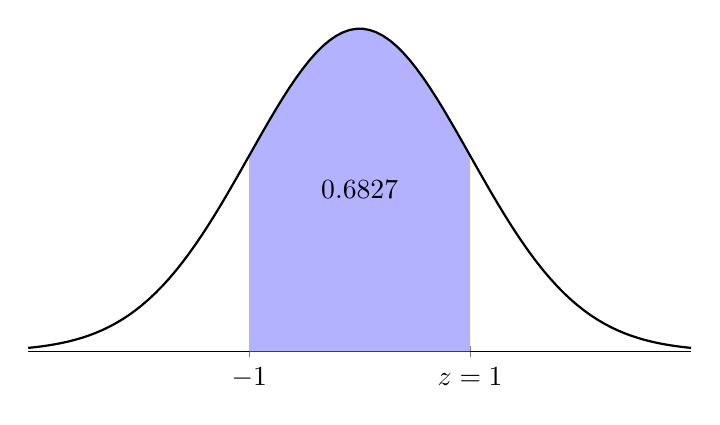
\begin{tikzpicture}
    \begin{axis}[
        no markers, 
        domain=-3:3, 
        samples=100,
        axis lines=left,
        height=6cm, width=10cm,
        xtick={-1, 1},
        xticklabels={$-1$, $z=1$},
        ytick=\empty,
        x axis line style={-},
        y axis line style={-},
        axis y line=none, % Remove the left y-axis spine
        xlabel near ticks,
        ylabel near ticks,
        ymin=0,
        ymax = 0.43
    ]
    
    \addplot [fill=blue!30, draw=none, domain=-1:1] {1/sqrt(2*pi)*exp(-x^2/2)} \closedcycle;
    \addplot [thick] {1/sqrt(2*pi)*exp(-x^2/2)};
    
    \node at (axis cs:0,0.2) {$0.6827$};
        
    \end{axis}
\end{tikzpicture}

\end{center}
\end{document}
